
\section{Estrutura do Robô} % (fold)
\label{sec:estrutura_do_robô}

Nesta seção pode-se visualizar os processos que levaram a construção da base do robô, componente responsável pela locomoção e a integração de todos os componentes. E as soluções que foram tomadas para a melhoria da construção baseadas em testes feitos com a estrutura.

\subsection{Fabricação}

Ocorreram, durante o processo de fabricação da estrutura, mudanças relacionadas ao material empregado na construção da base. A princípio, seria utilizado uma chapa de alumínio, porém foi verificado que a chapa de alumínio, além de possuir algumas dificuldades para serem usinadas e soldadas, deveria possuir uma espessura um pouco maior para não vibrar muito com a ação do sistema de sucção. Uma chapa de metal, mesmo sendo de alumínio, de 2 cm é extremamente pesada, o que se tornaria um problema para os sistemas de navegação e locomoção do robô. Por esse motivo, o alumínio foi substituído por uma chapa de aço de 2mm de espessura. A base construída possui 39 cm de diâmetro e uma área útil de 1100 cm$^2$, espaço suficiente para alocar todos os componentes do robô.

\begin{figure}[H]
	\centering
	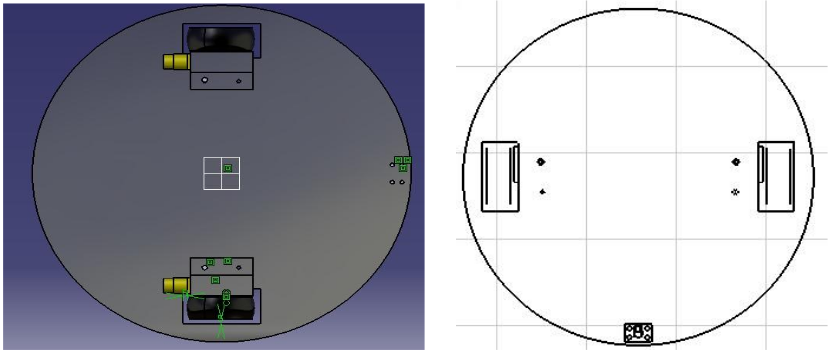
\includegraphics[scale=0.4]{figuras/vista_superior.png}
	\caption{Vista superior. A esquerda em 3D e a direita desenho técnico.}
	\label{img:vista_superior}
\end{figure}

O primeiro passo do processo de fabricação da estrutura foi a construção de um molde com as exatas dimensões da base, feito em madeira. Esse molde foi usado para verificar se o diâmetro de 39 cm seria suficiente para todos os componentes do robô e como seria feita a locação de cada componente, visando evitar erros no uso do material definitivo. Estando seguros do tamanho escolhido, foi feito o desenho circular em uma chapa de aço retangular utilizando um tipo de compasso, feito de prego e um lápis amarrado a uma linha de 20 cm. Em seguida, o corte circular foi feito com uma lixadeira. O diâmetro final da peça foi de 39 cm por causa da espessura da ferramenta que foi usada para o corte.

\begin{figure}[H]
	\centering
	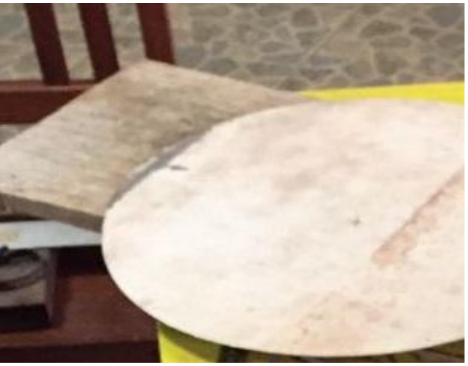
\includegraphics[scale=0.7]{figuras/primeiro_corte.png}
	\caption{Primeiro corte realizado para confecção da base.}
	\label{img:primeiro_corte}
\end{figure}

Com a base circular já pronta, foram feitas as marcações para os novos cortes e parafusos que entraram na estrutura, tudo isso, utilizando réguas e esquadros para se obter o melhor paralelismo possível para a peça final. Os cortes para o encaixe das rodas, foram feitos em formato retangular e exatamente do meio da peça. Para isso foi utilizado uma serra Tico Tico.

\begin{figure}[H]
	\centering
	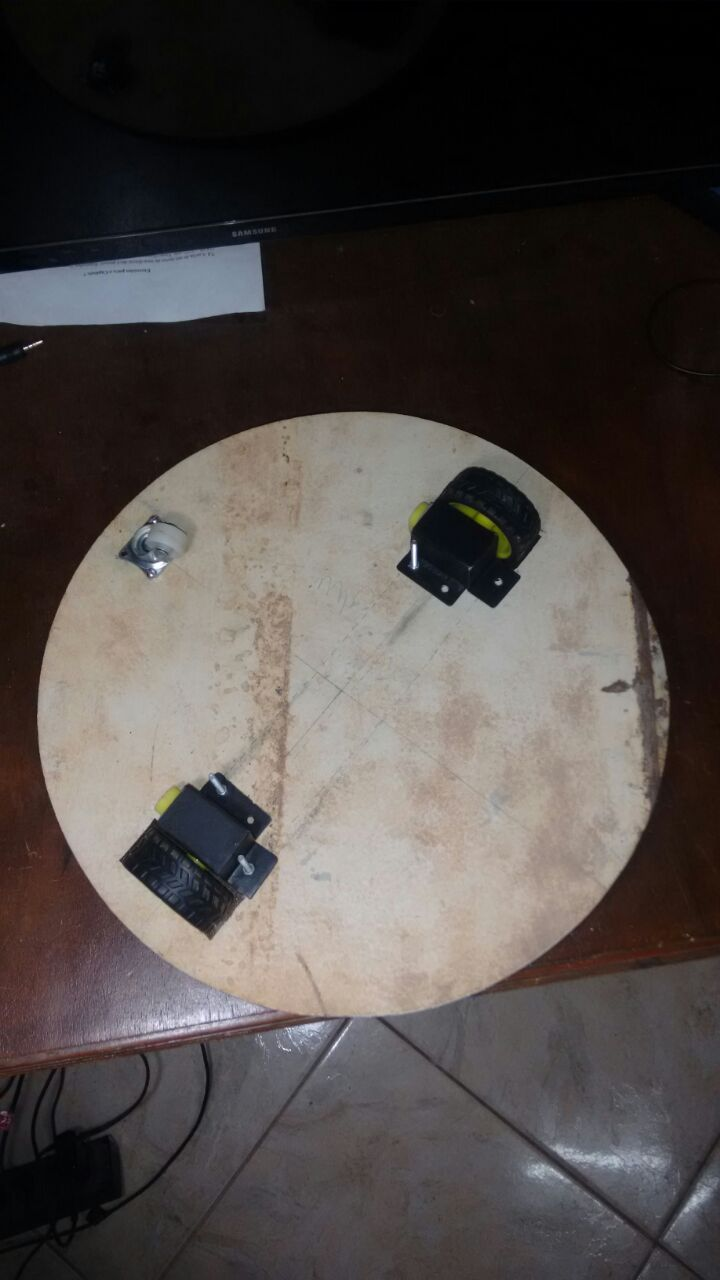
\includegraphics[scale=0.3]{figuras/serra_tico_tico.png}
	\caption{Base com as rodas montadas.}
	\label{img:serra_tico_tico}
\end{figure}

Tendo finalizado a estrutura principal da base, foi desenvolvido um suporte para fixar as rodas. Foram fabricados de tubo de aço retangular, “metalon”, de 30x25mm chapa 18. 

\begin{figure}[H]
	\centering
	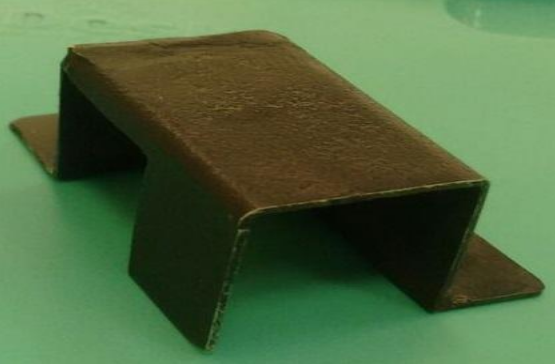
\includegraphics[scale=0.3]{figuras/suporte_fixar_rodas.png}
	\caption{Os suportes feitos para fixar as rodas.}
	\label{img:suporte_fixar_rodas}
\end{figure}

Com todos os componentes já produzidos, foram realizadas as furações na chapa com uma broca de 4mm para todos os parafusos e por fim os componentes foram montados e testados sua resistência e a capacidade de locomoção desse sistema. 

\begin{figure}[H]
	\centering
	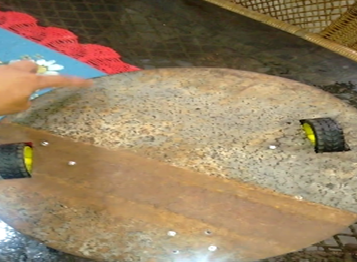
\includegraphics[scale=0.3]{figuras/base_teste.png}
	\caption{Teste 1 para verificar a estabilidade do carrinho.}
	\label{img:base_teste}
\end{figure}

Com o carrinho em movimento, a parte da estrutura que não possui roda livre era empurrada para baixo e se verificava o comportamento. Em todos os momentos o sistema voltava ao normal indicando que o uso de três rodas é viável dependendo da disposição dos componentes.

\begin{figure}[H]
	\centering
	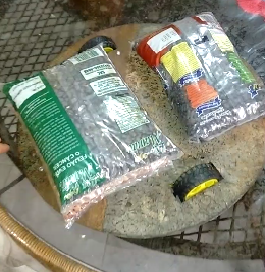
\includegraphics[scale=0.3]{figuras/base_teste_peso.png}
	\caption{Teste 2 – Verificando a resistência da estrutura.}
	\label{img:base_teste_peso}
\end{figure}

O teste consistia em colocar peso em cima da estrutura, aproximadamente 2 kg, e se empurrou o carrinho para ver seu comportamento.

\section{Documentação em CAD}

Durante o processo de fabricação da estrutura ocorreram alguns retrabalhos na documentação feita no CATIA, alguns sketches feitos eram mais complicados de serem usinados e poderiam nos trazer diversos erros de paralelismo na estrutura. Os desenhos finais da estrutura da base do motor são apresnetados a seguir.

\begin{figure}[H]
	\centering
	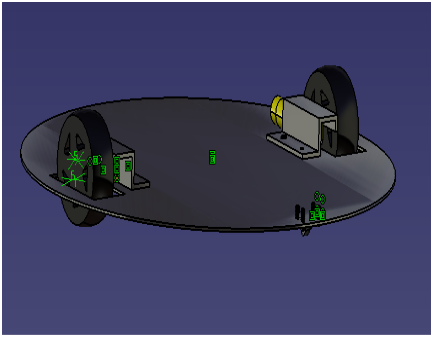
\includegraphics[scale=0.3]{figuras/vista_isometrica.png}
	\caption{Vista isométrica.}
	\label{img:vista_isometrica}
\end{figure}

\begin{figure}[H]
	\centering
	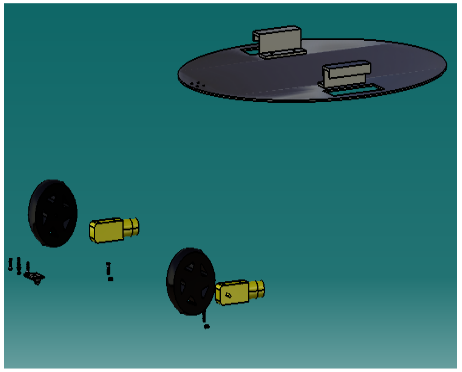
\includegraphics[scale=0.3]{figuras/vista_explodida.png}
	\caption{Vista explodida dos componentes.}
	\label{img:vista_explodida}
\end{figure}

\begin{figure}[H]
	\centering
	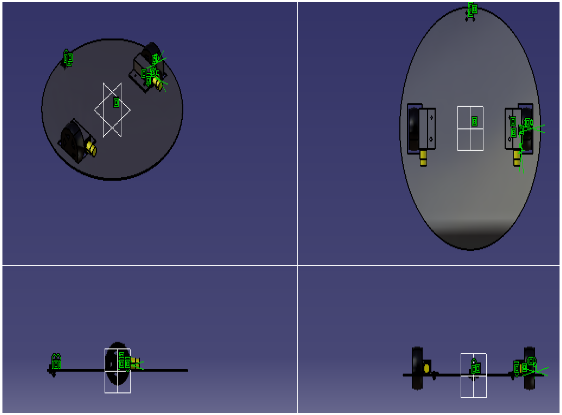
\includegraphics[scale=0.3]{figuras/vistas_em_corte.png}
	\caption{Vistas em corte.}
	\label{img:vistas_em_corte}
\end{figure}
% section estrutura_do_robô (end)